
\documentclass[8pt, t, aspectratio=169,% for widescreen (16:9) presentations
%aspectratio=43,% for traditional (4:3) presentations
%handout%
]{beamer}

\usepackage{tabularx}
\usepackage{color}

%%%%%%%%%%%%%%%%%%%%%%%%%%%%%%%%%% mode options %%%%%%%%%%%%%%%%%%%%%%%%%%%%%%%%

\mode<presentation>{\usetheme{uniS}}

% define a few pictures used throughout the slides
\pgfdeclareimage[height=1.01\paperheight]{background}{./images/titelbild.jpg}  % background picture for title slide
\pgfdeclareimage[height=1cm]{unilogo}{unilogo.pdf} % UniS logo for title slide
\pgfdeclareimage[height=1cm]{unilogow}{unilogo_w.pdf} % (white) UniS logo for final slide
\pgfdeclareimage[width=2.5cm]{speaker}{speaker.jpg} % speaker photo for final slide


%%%%%%%%%%%%%%%%%%%%%%%%%%%%%%%%%% misc stuff %%%%%%%%%%%%%%%%%%%%%%%%%%%%%%%%%%

% automatically display \sectionpage at beginning of every \section{}
\AtBeginSection[]{%
\begin{frame}[plain]
  \sectionpage
\end{frame}
% uncomment block in order to display toc after every sectionpage
%\usepackage{multicol}
%\begin{frame}[c, plain]
%  \begin{footnotesize}
%    \begin{center}
%      \begin{minipage}{.75\textwidth}
%        \begin{multicols}{2}
%          \tableofcontents[currentsection]
%        \end{multicols}
%      \end{minipage}
%    \end{center}
%  \end{footnotesize}
%\end{frame}
}
\usepackage{tikz}
\usetikzlibrary{shapes.geometric, arrows, calc}
% Define block styles
%\tikzstyle{startstop} = [rectangle, rounded corners, minimum width=3cm, minimum height=1cm,text centered, draw=black, fill=red!30]
%\tikzstyle{io} = [trapezium, trapezium left angle=70, trapezium right angle=110, minimum width=2cm, minimum height=1cm, text centered, draw=black, fill=blue!30]
%\tikzstyle{process} = [rectangle, minimum width=3cm, minimum height=1cm, text centered, text width=3cm, draw=black, fill=orange!30]
%\tikzstyle{decision} = [diamond, minimum width=3cm, minimum height=1cm, text centered, draw=black, fill=green!30]
%\tikzstyle{arrow} = [thick,->,>=stealth]

\tikzstyle{startstop} = [rectangle, rounded corners, minimum width=3cm, minimum height=0.5cm,text centered, draw=black]
\tikzstyle{io} = [trapezium, trapezium left angle=70, trapezium right angle=110, minimum width=2cm, minimum height=0.5cm, text centered, draw=black]
\tikzstyle{process} = [rectangle, minimum width=3cm, minimum height=0.5cm, text centered, text width=3cm, draw=black]
\tikzstyle{processLarge} = [rectangle, minimum width=3cm, minimum height=0.5cm, text centered, text width=6cm, draw=black]
\tikzstyle{decision} = [diamond, minimum width=2cm, minimum height=0.5cm, text centered, draw=black]
\tikzstyle{arrow} = [thick,->,>=stealth]


%%%%%%%%%%%%%%%%%%%%%%%%%%%%%%%%%%%% setup %%%%%%%%%%%%%%%%%%%%%%%%%%%%%%%%%%%%%

\title{Modul 7: \\ Levenberg-Marquardt \\ Algorithmus}
\author[Florian Gschwandtner]{Florian \\ Gschwandtner}
\institute{IFR}

%%%%%%%%%%%%%%%%%%%%%%%%%%%%%%%%%%% slides %%%%%%%%%%%%%%%%%%%%%%%%%%%%%%%%%%%%%

\begin{document}

\begin{frame}[plain]
  \titlepage
\end{frame}


\section{Überblick} % Section title slide, unnumbered

\begin{frame}{Themen}
	\begin{itemize}\huge
		\item[]	1. Überblick
		\item[] 2. Problemstellung
		\item[] 3. Algorithmus
		\item[] 4. Anwendungsbeispiel
		\item[] 5. Zusammenfassung
%		\item[] 6. Anwendung im Regelkreis
%		\item[] 7. Zusammenfassung und Ausblick
	\end{itemize}

\end{frame}

%----------------------------------------------------------------------------------------

\section{Problemstellung}

\begin{frame}{Nichtlineare Optimierung}\LARGE

Modell
\begin{equation}
	\textbf{z} =  f(\hat{\textbf{x}})+\textbf{e}
\end{equation}

\begin{itemize}
	\item Mindestens einmal stetig differenzierbar
	\item Erste Ableitung stetig
\end{itemize}

Abweichung
\begin{equation}
	\Delta \textbf{y}_c = \textbf{z}-\textbf{f}(\textbf{x}_c)
\end{equation}\label{deltayc}


Kostenfunktion
\begin{equation}
	J_c = \Delta \textbf{y}_c^T W \Delta \textbf{y}_c
\end{equation}\label{jc}

\end{frame}

\begin{frame}{Gradientenverfahren}\LARGE

\begin{equation}
	\Delta\textbf{x}_{grad} = \frac{1}{\eta}\textbf{H}^T\textbf{W}\Delta\textbf{y}_c
\end{equation}

\begin{minipage}{0.5\linewidth}
Vorteile
\begin{itemize}
	\item Abnahme in steilste Richtung der Kostenfunktion
	\item Mit Schrittweitensteuerung großer Konvergenzbereich
\end{itemize}
\end{minipage}%
\begin{minipage}{0.5\linewidth}
Nachteile
\begin{itemize}
	\item Langsame Konvergenz nahe dem Minimum
	\item Stark Abhängig von der Schrittweite
\end{itemize}
\end{minipage}
\end{frame}



\begin{frame}{Gauss-Newtonverfahren}\LARGE
\begin{equation}
	\Delta \textbf{x}_{LSQ} = (\textbf{H}^T \textbf{W} \textbf{H})^{-1} \textbf{H}^T \textbf{W} \Delta \textbf{y}_c
\end{equation}

\begin{minipage}{0.5\linewidth}
Vorteile
\begin{itemize}
	\item Schnelle Konvergenz
	\item Anwendungsbereich
\end{itemize}
\end{minipage}%
\begin{minipage}{0.5\linewidth}
Nachteile
\begin{itemize}
	\item Abhängig vom Startwert
	\item Unzuverlässige Konvergenz
\end{itemize}
\end{minipage}

\end{frame}


\section{Levenberg-Marquart Algorithmus}

\begin{frame}{Iterationsvorschrift} \LARGE
	\begin{equation}
		\Delta\textbf{x}=(\textbf{H}^T \textbf{W} \textbf{H}+\eta \mathcal{H})^{-1}\textbf{H}^T \textbf{W} \Delta \textbf{y}_c
	\end{equation}


mit

\begin{equation}
	\textbf{H} =  \frac{\partial \textbf{f}}{\partial \textbf{x}}\big|_{\textbf{x}_c}
\end{equation}

und
\begin{equation}
	\mathcal{H} = \textbf{I} \: oder \: Diagonalelemente \: von \: \textbf{H}^T\textbf{WH}
\end{equation}
%\begin{itemize}
%	\item 
%\end{itemize}
	
\end{frame}

\begin{frame}{Ablauf}

\centering
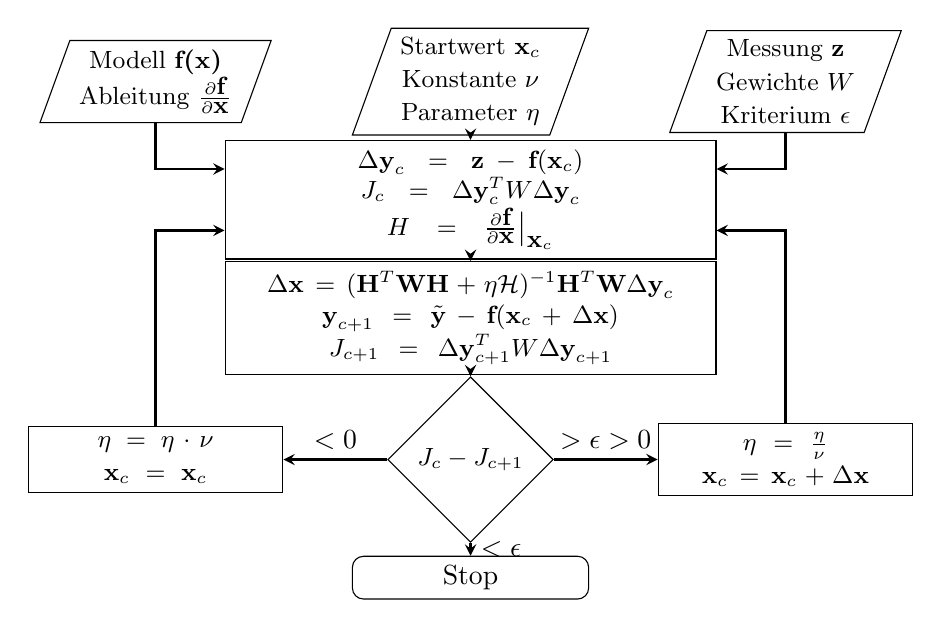
\begin{tikzpicture}[node distance=1cm]

	\node (inModel) [io, align=center] {\small Modell $\textbf{f(x)}$  \\ \small Ableitung $\frac{\partial \textbf{f}}{\partial \textbf{x}}$};
%	\node (H) [process, below of=inModel] {Bestimme };  
	\node (inStart) [io, right of=inModel, xshift=3cm, align=center] {\small Startwert $\textbf{x}_c$ \\ \small Konstante $\nu$ \\ \small Parameter $\eta$};
	\node (inStart2) [io, right of=inStart, xshift=3cm, align=center] {\small  Messung $\textbf{z}$ \\ \small Gewichte $W$ \\ \small Kriterium $\epsilon$};

	%\node (inny) [io, right of=inStart, xshift=3cm] {Konstante $\nu$};

	\node (calcPro) [processLarge, below of=inStart, yshift=-0.5cm] {\small $\Delta \textbf{y}_c = \textbf{z}-\textbf{f}(\textbf{x}_c)$ \\ $J_c = \Delta \textbf{y}_c^T W \Delta \textbf{y}_c$ \\ $H = \frac{\partial \textbf{f}}{\partial \textbf{x}}\big|_{\textbf{x}_c}$};
	
	%\node (deltaXPro)[processLarge, below of=calcPro] {\small $\Delta\textbf{x}=(\textbf{H}^T \textbf{W} \textbf{H}+\eta \mathcal{H})^{-1}\textbf{H}^T \textbf{W} \Delta \textbf{y}_c$};
	\node (Jc1Pro)[processLarge, below of=calcPro,yshift=-0.5cm] {\small $\Delta\textbf{x}=(\textbf{H}^T \textbf{W} \textbf{H}+\eta \mathcal{H})^{-1}\textbf{H}^T \textbf{W} \Delta \textbf{y}_c$ \\ \small $\textbf{y}_{c+1} = \tilde{\textbf{y}}-\textbf{f}(\textbf{x}_c+\Delta \textbf{x}) $ \\ \small $J_{c+1} = \Delta \textbf{y}_{c+1}^T W \Delta \textbf{y}_{c+1}$};

	\node (decJ) [decision, below of=Jc1Pro, yshift=-0.8cm] {\small $J_c-J_{c+1}$};
	\node (larger) [process, right of=decJ, xshift=3cm] {\small $\eta = \frac{\eta}{\nu}$ \\ \small $\textbf{x}_c = \textbf{x}_c+\Delta \textbf{x}$};
	\node (smaller) [process, left of=decJ, xshift=-3cm] {\small $\eta = \eta \cdot \nu$ \\ \small $\textbf{x}_c = \textbf{x}_c$};
	\node (stop) [startstop, below of=decJ, yshift=-0.5cm] {Stop};
	
%	\draw [arrow] (inModel)--(H);
	\draw [arrow] (inModel)|-([yshift=0.5cm]calcPro);
	\draw [arrow] (inStart)--(calcPro);
	\draw [arrow] (inStart2)|-([yshift=0.5cm]calcPro);
	\draw [arrow] (calcPro)--(Jc1Pro);
	%\draw [arrow] (deltaXPro)--(Jc1Pro);
	
	\draw [arrow] (Jc1Pro)--(decJ);
	\draw [arrow] (decJ)--node[anchor=south] {$>\epsilon>0$}(larger);
	\draw [arrow] (decJ)--node[anchor=south] {$<0$}(smaller);
	\draw [arrow] (decJ)--node[anchor=west] {$<\epsilon$}(stop);	
	
	\draw [arrow] (larger)|-([yshift=-0.5cm]calcPro);
	\draw [arrow] (smaller)|-([yshift=-0.5cm]calcPro);
\end{tikzpicture}

\end{frame}

\begin{frame}{Wahl der Konstanten} \LARGE

Schrittweite $\eta$
	\begin{equation}
		\eta \approx 10 \; bis \; 100 \cdot ||\textbf{H}^T  \textbf{W} \textbf{H}||_2 \approx 10^6 \; bis \; 10^8
	\end{equation}

\vspace{2cm}

Konstante $\nu$
	\begin{equation}
		\nu \approx 2 \; bis \; 10 
	\end{equation}
\end{frame}

%\begin{frame}{Verwendete Form}
%
%	\Huge
%	\begin{equation*}
%	P(s) = K_p\cdot \frac{T_L\cdot s+1}{T_l\cdot s+1}\cdot e^{-\tau_e\cdot s}
%	\end{equation*}
%
%	\vspace{1.5cm}	
%	
%	\large
%	\begin{tabularx}{\textwidth}{ll}
%	$K_p$ & \qquad Verstärkungsfaktor \\
%	$T_L$ & \qquad Zeitkonstante der Nullstelle \\
%	$T_l$ & \qquad Zeitkonstante des Pols\\
%	$\tau_e$ & \qquad Effektive Zeitverzögerung \\
%	\end{tabularx}
%
%\end{frame}

%------------------------------------------------

\section{Anwendungsbeispiel}



\begin{frame}{Modell (1)}

Form
\begin{equation}
	f(x,y) = a \cdot (x-a)^3+100\cdot e^{b\cdot(x^2+y^2)}
\end{equation}


Messwerte
\begin{equation}
	\textbf{z} = 0,5 \cdot (x-0,5)^3+100\cdot e^{-0,2\cdot(x^2+y^2)}+10*(rand()-0.5) 
\end{equation}

\centering
\begin{minipage}{0.5\linewidth}
	\centering
	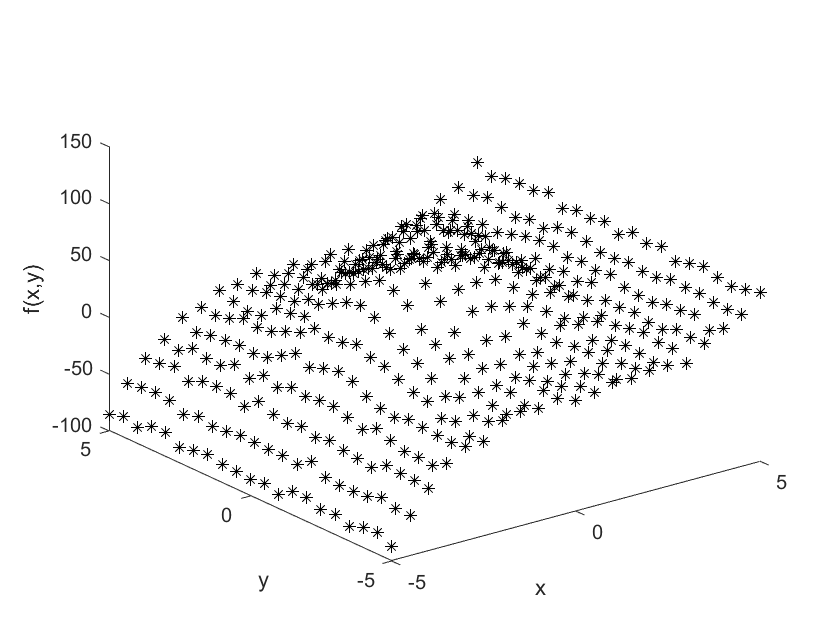
\includegraphics[width=0.9\linewidth]{./Images/daten.png}
\end{minipage}%
\begin{minipage}{0.5\linewidth}
	\centering
	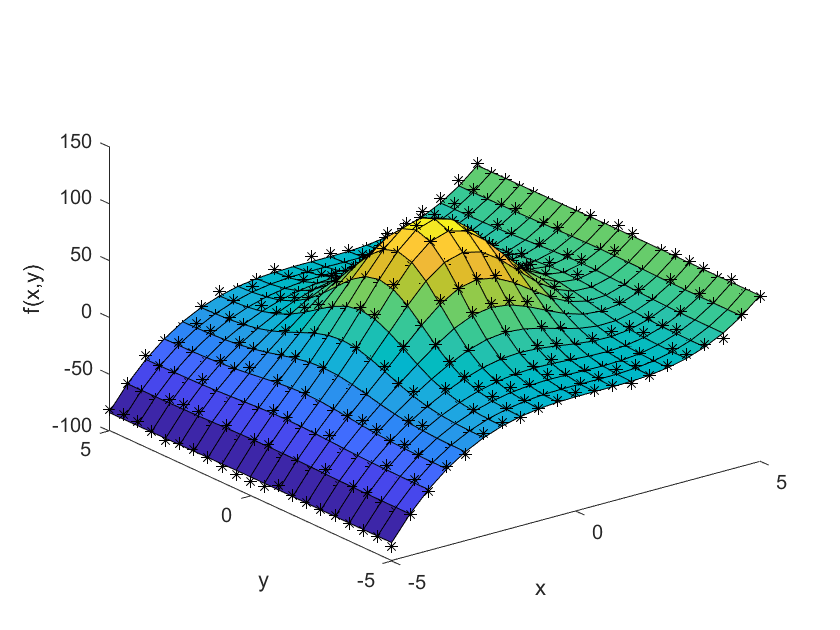
\includegraphics[width=0.9\linewidth]{./Images/result.png}
\end{minipage}
\end{frame}

\begin{frame}{Modell (2)}

Jacobimatrix
\begin{equation}
	\textbf{H}=
	\begin{bmatrix}
		(x_1-a)^3+3 \cdot a \cdot (x_1-a)^2 & (x_1^2+y_1^2)\cdot e^{b \cdot (x_1^2+y_1^2)}\\
		(x_2-a)^3+3 \cdot a \cdot (x_2-a)^2 & (x_2^2+y_1^2)\cdot e^{b \cdot (x_2^2+y_1^2)}\\
			\cdot&\cdot \\
			\cdot&\cdot \\
		(x_k-a)^3+3 \cdot a \cdot (x_k-a)^2 & (x_k^2+y_1^2)\cdot e^{b \cdot (x_k^2+y_1^2)}\\
		(x_1-a)^3+3 \cdot a \cdot (x_1-a)^2 & (x_1^2+y_2^2)\cdot e^{b \cdot (x_1^2+y_2^2)}\\
			\cdot&\cdot \\
			\cdot&\cdot \\
	 	(x_k-a)^3+3 \cdot a \cdot (x_k-a)^2 & (x_k^2+y_j^2)\cdot e^{b \cdot (x_k^2+y_j^2)}\\	
	\end{bmatrix}
\end{equation}

Gewichte
\begin{equation}
	\textbf{W}=I
\end{equation}



%Messwerte
%\begin{equation}
%	\tilde{\textbf{y}} = 0,5 \cdot (x-0,5)^3+100\cdot e^{-0,2\cdot(x^2+y^2)}+10*(rand()-0.5) 
%\end{equation}
\end{frame}



\begin{frame}{Gauss-Newton Verfahren}

\centering
\begin{minipage}{0.5\linewidth}
	\centering
	\includegraphics[width=0.9\linewidth]{./Images/JPlotLSQ.png}
\end{minipage}%
\begin{minipage}{0.5\linewidth}
	\centering
	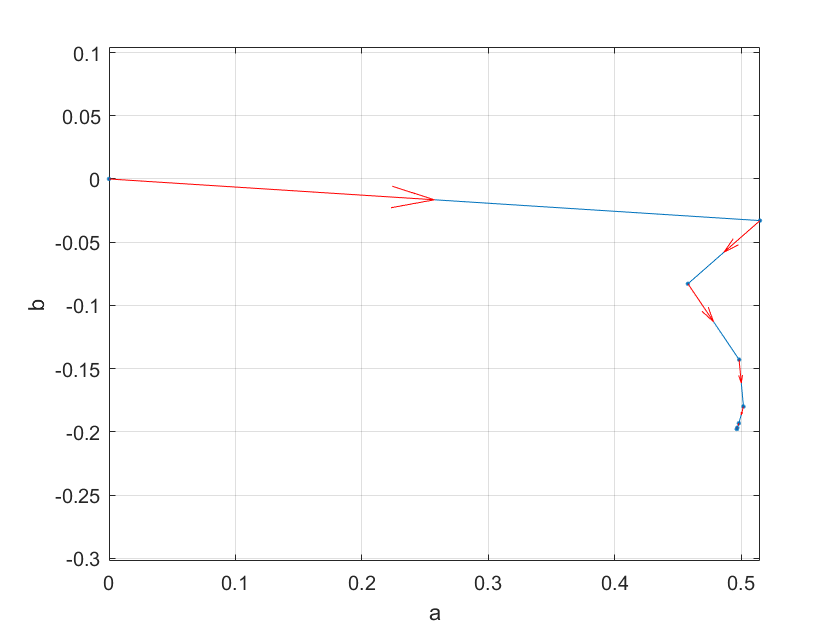
\includegraphics[width=0.9\linewidth]{./Images/abVerlaufLSQ.png}
\end{minipage}
\end{frame}


\begin{frame}{Gradientenverfahren}

\centering
\begin{minipage}{0.5\linewidth}
	\centering
	\includegraphics[width=0.9\linewidth]{./Images/JPlotGrad.png}
\end{minipage}%
\begin{minipage}{0.5\linewidth}
	\centering
	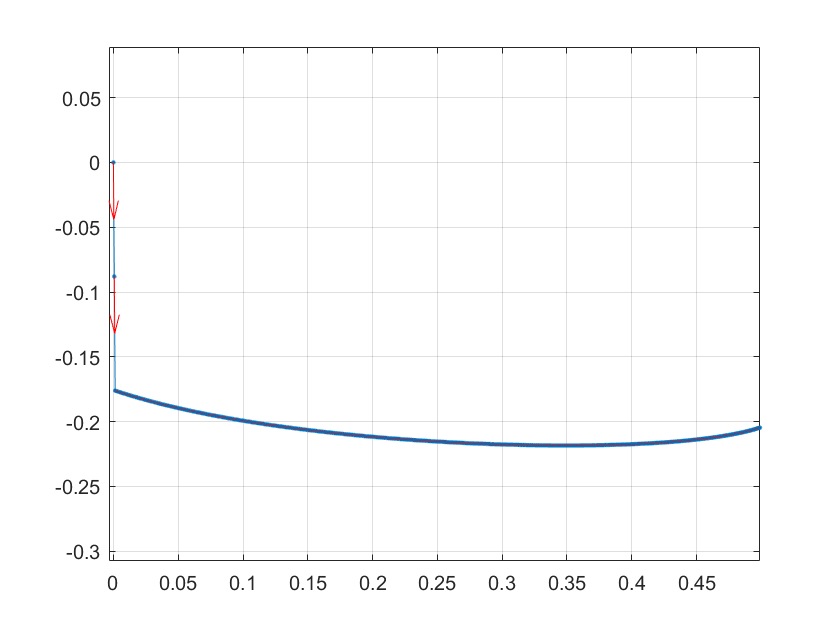
\includegraphics[width=0.9\linewidth]{./Images/abVerlaufGrad.png}
\end{minipage}
\end{frame}

\begin{frame}{Levenberg-Marquardt Verfahren - Kostenfunktion}

\centering
\begin{minipage}{0.5\linewidth}
	\centering
	\includegraphics[width=0.9\linewidth]{./Images/JPlot.png}
\end{minipage}%
\begin{minipage}{0.5\linewidth}
	\centering
	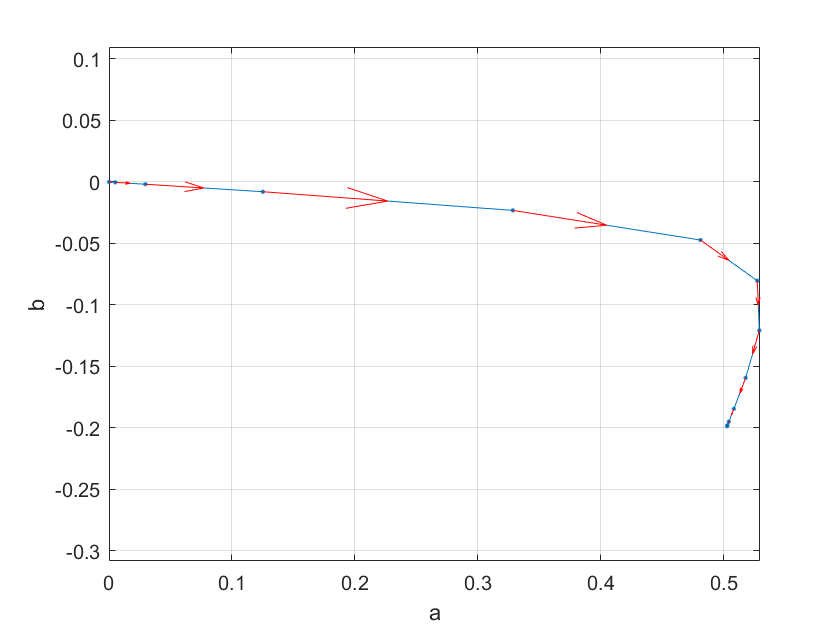
\includegraphics[width=0.9\linewidth]{./Images/abVerlauf.png}
\end{minipage}
\end{frame}


\begin{frame}{Levenberg-Marquardt Verfahren - $\eta$}

\centering
\begin{minipage}{0.5\linewidth}
	\centering
	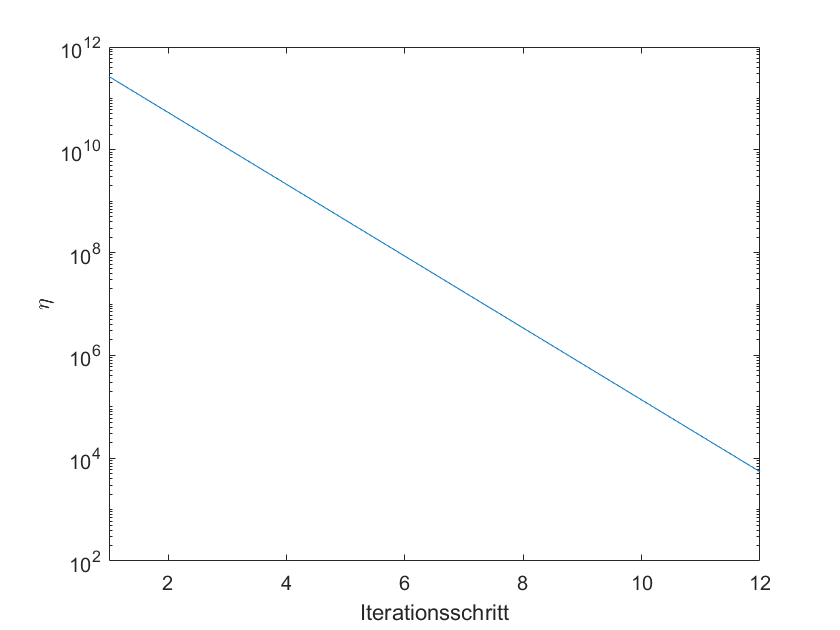
\includegraphics[width=0.9\linewidth]{./Images/eta.png}
\end{minipage}%
%\begin{minipage}{0.5\linewidth}
%	\centering
%	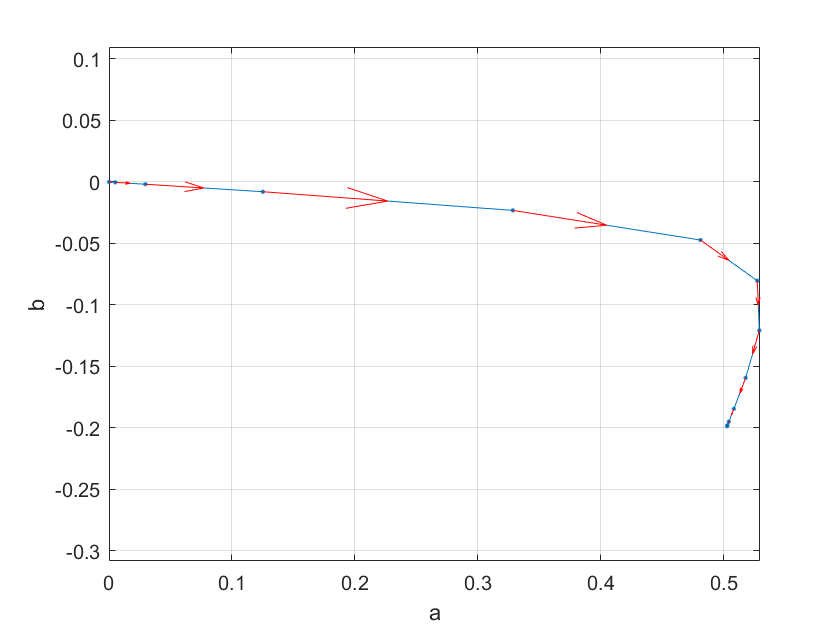
\includegraphics[width=0.9\linewidth]{./Images/abVerlauf.png}
%\end{minipage}
\end{frame}

\begin{frame}{Konvergenz}

\centering
\begin{tabular}{|l|l|c|c|c|}

\hline
$a_0$& $b_0$& Levenberg-Marquardt & Newton & Gradient  \\
\hline
\hline
$-10$& $-10$& $X $ & $X $ & $X$ \\
\hline
$-5$& $-5$& $\checkmark (16)$ & $X $ & $X $ \\
\hline
$-5$& $0$& $\checkmark (13)$ & $\checkmark (8) $ & $X $ \\
\hline
$0$& $5$ & $\checkmark (9)$ & $X $ & $X $ \\
\hline
$-2$& $-2$ &  $\checkmark (45)$ & $X $ & $X $ \\
\hline
$-1$& $-1$ &  $\checkmark (9)$ & $\checkmark (6) $ &  $\checkmark (4773) $ \\
\hline
$0$& $0$ & $\checkmark (13)$ & $\checkmark (9) $ & $\checkmark (2784) $ \\
\hline
$0$& $2$  & $\checkmark (21)$ & $X $ & $X $ \\
\hline
$2$& $0$  & $\checkmark (12)$ & $\checkmark (7) $ & $X $ \\
\hline
$2$& $2$  & $\checkmark (43)$ & $X $ & $X $ \\
\hline
$5$& $2$  & $\checkmark (42)$ & $X $ & $X $ \\
\hline
$5$& $5$  & $X $ & $X $ & $X$ \\
\hline


\end{tabular}
\end{frame}


%\begin{frame}{Parameterfindung}
%
%
%\end{frame}

%------------------------------------------------

\section{Zusammenfassung}

\begin{frame}{Zusammenfassung}\LARGE
	\begin{itemize}
		\item Konvergenzbereich stark erhöht
		\item Rechenaufwand moderat höher
		\item Wahl von $\eta$ und $\nu$
		\begin{itemize}
			\item $\eta \approx 10 \; bis \; 100 \cdot ||\textbf{H}^T  \textbf{W} \textbf{H}||_2 \approx 10^6 \; bis \; 10^8$
			\item $\nu \approx 2 \; bis \; 10 $
		\end{itemize}
	\end{itemize}
\end{frame}
%------------------------------------------------

%%%%%%%%%%%%%%%%%%%%%%%%%%%%%%%%% final slide %%%%%%%%%%%%%%%%%%%%%%%%%%%%%%%%%%
\finalslide{<<email>>}{<<tel>>}{<<fax>>}

\end{document}
